%%%%%%%%%%%%%%%%%%%%%%%%%%%
% Práctica 7: Persistencia de datos
% @uthor: Alejandro David Arzola Saavedra
% @date: 04/11/2023
%%%%%%%%%%%%%%%%%%%%%%%%%%%
% Estructura basica de la pagina
\documentclass[a4paper]{article}
\usepackage[utf8]{inputenc}
\usepackage[spanish]{babel}
\usepackage{fancyhdr} %Definimos el estilo de página

% Paquetes adicionales
\usepackage{graphicx,efbox}
\usepackage[headsep=0.2cm]{geometry}
\usepackage[most]{tcolorbox}
\newcommand{\MYhref}[3][black]{\href{#2}{\color{#1}{#3}}}
\usepackage[hyperindex=true, colorlinks=true, linkcolor=black, breaklinks=true, urlcolor=black, citecolor=black, anchorcolor= black]{hyperref}

\usepackage{hyperref}

% Configuración del color del enlace
\hypersetup{
  colorlinks=true,
  linkcolor=blue, % Color azul
  urlcolor=blue,  % Color azul para enlaces URL
  citecolor=blue  % Color azul para citas
}

\hypersetup{
  linkcolor=black, % Cambiar a negro
}

% Agrega el paquete para personalizar el índice
\usepackage{tocloft}

% Personaliza la apariencia de la entrada "Bibliografía" en el índice
\renewcommand{\cftsecleader}{\cftdotfill{\cftdotsep}}
\renewcommand{\cftsecafterpnum}{\vspace{0.5\baselineskip}}

% Variable de entorno de fecha
\newcommand{\dateToday}{04 de noviembre de 2023}

% Variable de imagenes
\newcommand{\logoULPGC}{imagenes/ulpgc.png}
\newcommand{\android}{imagenes/android.png}
\newcommand{\androidStudio}{imagenes/android_studio.png}
\newcommand{\busAppMaster}{imagenes/busAppView.png}
\newcommand{\busAppView}{imagenes/busAppMaster.png}
\newcommand{\plantViewCircle}{imagenes/plantViewCircle.png}
\newcommand{\plantViewColumn}{imagenes/plantViewColumn.png}
\newcommand{\plantViewGrid}{imagenes/plantViewGrid.png}
%Cambio indice
\addto\captionsspanish{\renewcommand{\contentsname}{Índice}}

\setlength{\headheight}{ 40.2pt}
\pagestyle{fancy}
\lhead{\includegraphics[width=5cm]{\logoULPGC}}\rhead{
\includegraphics[height=1cm]{imagenes/android-icon.png}}

\geometry{a4paper, total={170mm,257mm}, left=35mm, top=20mm, right=35mm}

\begin{document}
    %%%%%%%%%%%%%%%%%%%%%%%%%%%%%%%%%
    %%   Portada del documento
    %%%%%%%%%%%%%%%%%%%%%%%%%%%%%%%%%
    \begin{titlepage}
        \centering
        \vspace*{2cm}
        \includegraphics[width=0.6\textwidth]{\logoULPGC}\par\vspace{1cm}
    
        {\scshape\textbf{\LARGE Práctica 6}}\par
        \vspace{0.6cm}
        {\bfseries}{\Huge Persistencia de datos}
        \vspace{2cm}
    
        \centering
        
\includegraphics[width=0.8\textwidth, keepaspectratio]{\android}
        \vspace{0.5cm}\vspace{0.5cm}
        \begin{tcolorbox}[colback=red!5!white,colframe=white!50!black]
            \centering \Large Programación de Aplicaciones Móviles Nativas \par
            \dateToday
        \end{tcolorbox}

        \vspace{1cm}        
        \begin{tcolorbox}[colback=blue!5!white,colframe=blue!75!black]
            Autor:
            \tcblower
            Alejandro David Arzola Saavedra (alejandro.arzola101@alu.ulpgc.es)
        \end{tcolorbox}
    \end{titlepage}
    
    \newpage
        
    %%%%%%%%%%%%%%%%%%%%%%%%%%%%%%%%%
    % Tabla de contenido de la pagina
    %%%%%%%%%%%%%%%%%%%%%%%%%%%%%%%%%
    \tableofcontents 
    
    \newpage

    %%%%%%%%%%%%%%%%%%%%%%%%%%%
    % Introduccion de la pagina
    %%%%%%%%%%%%%%%%%%%%%%%%%%%
    \section{Introducción}

    Esta sección se enfoca en la Unidad 6: "\textbf{Persistencia de datos}" dentro de la ruta de aprendizaje de Aspectos Básicos de Android con Compose. \vspace{0.3cm}
    
    Los temas clave que se abordarán en esta unidad son los siguientes:

    \begin{itemize}
    \item Introducción a SQL:
    En esta parte, se proporcionará una \textbf{introducción a SQL} (Structured Query Language).

    \item Cómo usar Room para lograr la persistencia de datos:
    Se explorará el uso de la biblioteca \textbf{Room} para facilitar la creación y utilización de bases de datos relacionales en una aplicación para Android.

    \item Cómo almacenar datos y acceder a ellos mediante claves con DataStore:
    La última parte de esta unidad se centrará en aprender a \textbf{almacenar datos simples} utilizando el componente \textbf{Preferences Datastore}.

    \end{itemize}
    
    \section{Enlace Github}
    % Enlace al repositorio de Git con el CodeLab
    El enlace al repositorio de GitHub es el siguiente:\vspace{0.3cm}
    
    \href{https://github.com/AlejandroDavidArzolaSaavedra/Bus-Stop-List-app}{Clicka aqui para ver la Bus APP usando ROOM en Github}\vspace{0.3cm}

    El enlace al repositorio de GitHub es el siguiente:\vspace{0.3cm}

    \href{https://github.com/AlejandroDavidArzolaSaavedra/Plant-Kingdom-app}{Clicka aqui para ver la Plant-Kingdom APP usando ROOM y DataStore en Github}\vspace{0.3cm}
    
    
    \section{Capturas del Emulador}
    \subsection{Aplicacion simple usando Room}
    \begin{figure}[h]
        \begin{center}
        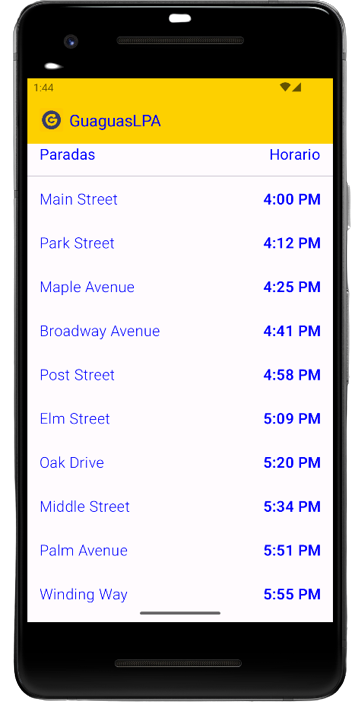
\includegraphics[width=0.5\textwidth, height=8cm, keepaspectratio]{\busAppMaster}
        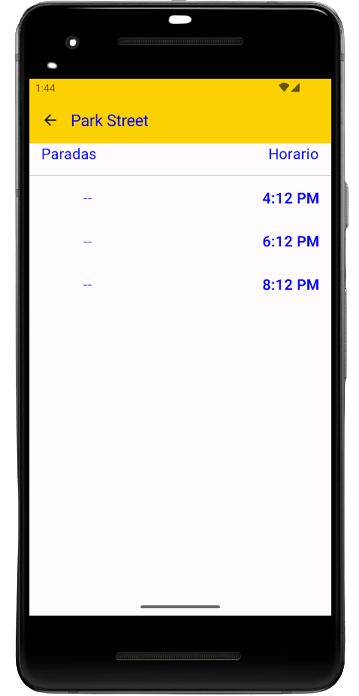
\includegraphics[width=0.5\textwidth, height=8cm, keepaspectratio]{\busAppView}
        \end{center}
        \textbf{\caption{Aplicacion de Guaguas usando ROOM}}
    \end{figure}
    
    \subsection{Aplicacion simple usando DataStore}
        \begin{figure}[h]
        \begin{center}
        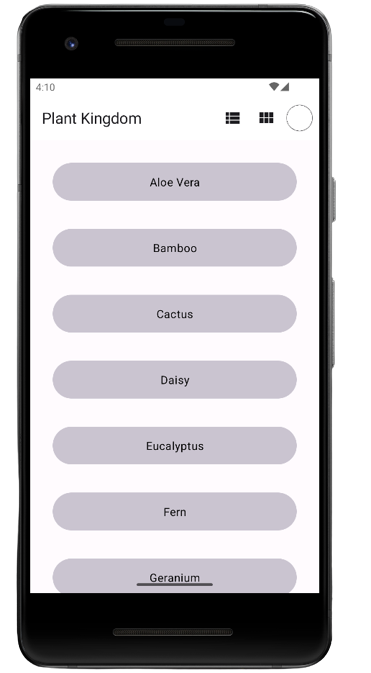
\includegraphics[width=0.33\textwidth, height=8cm, keepaspectratio]{\plantViewCircle}
        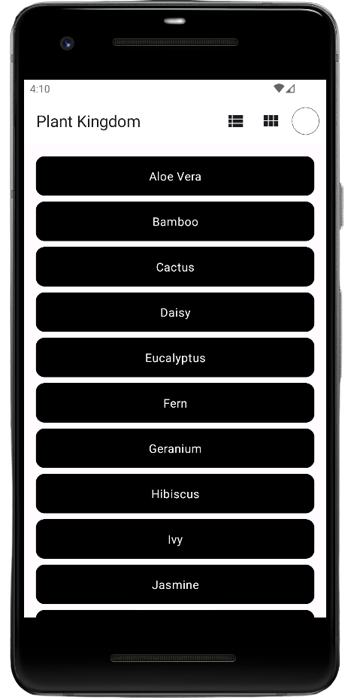
\includegraphics[width=0.33\textwidth, height=8cm, keepaspectratio]{\plantViewColumn}
        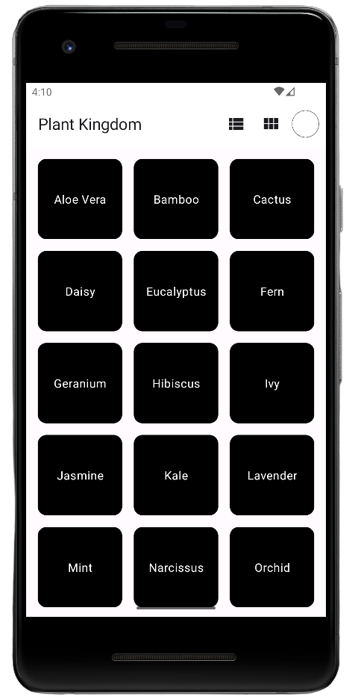
\includegraphics[width=0.33\textwidth, height=8cm, keepaspectratio]{\plantViewGrid}
        \end{center}
        \textbf{\caption{Aplicacion Reino de plantas usando Datastore}}
    \end{figure}
    \section{Opinión del Codelab}
   
    En mi perspectiva, este codelab fue \textbf{considerablemente más extenso y complejo que el anterior}. En algunas instancias, me vi obligado a retroceder en la documentación, ya que se daban por sentados conceptos que no tenía completamente claros. Sin embargo, la complejidad adicional ofreció una oportunidad para profundizar en conceptos más avanzados de persistencia de datos en el entorno de desarrollo Android.\vspace{0.3cm}
    
    Durante la realización de la práctica, pude comprender en detalle cómo utilizar \textbf{Room} para gestionar bases de datos relacionales en una aplicación Android. La introducción a SQL proporcionada en la unidad era basica, pero nunca viene mal refrescar conceptos.\vspace{0.3cm}
    
    Además, la sección que aborda el almacenamiento y acceso de datos mediante claves con \textbf{DataStore} amplió mi comprensión sobre las opciones disponibles para \textbf{persistir datos} simples de manera eficiente.\vspace{0.3cm}

    
\end{document}